%%%%%%%%%%%%%%%%%%%%%%%%%%%%%%%%%%%%%%%%%%%%%%%%%%%%%%%%
\documentclass[12pt,a4paper]{article}% 文档格式
\usepackage{ctex,hyperref}% 输出汉字
\usepackage{times}% 英文使用Times New Roman
%%%%%%%%%%%%%%%%%%%%%%%%%%%%%%%%%%%%%%%%%%%%%%%%%%%%%%%%
\title{\fontsize{18pt}{27pt}\selectfont% 小四字号,1.5倍行距
{\heiti% 黑体
Monte Calo 的收敛阶数讨论}}% 题目
%%%%%%%%%%%%%%%%%%%%%%%%%%%%%%%%%%%%%%%%%%%%%%%%%%%%%%%%
\author{\fontsize{12pt}{18pt}\selectfont% 小四字号,1.5倍行距
{\fangsong% 仿宋
白博臣、何骐多、夏营}\\% 标题栏脚注
\fontsize{10.5pt}{15.75pt}\selectfont% 五号字号,1.5倍行距
{\fangsong% 仿宋
(四川大学~~~物理学拔尖计划)}}% 作者单位,“~”表示空格
%%%%%%%%%%%%%%%%%%%%%%%%%%%%%%%%%%%%%%%%%%%%%%%%%%%%%%%%
\date{}% 日期(这里避免生成日期)
%%%%%%%%%%%%%%%%%%%%%%%%%%%%%%%%%%%%%%%%%%%%%%%%%%%%%%%%
\usepackage{amsmath,amsfonts,amssymb}% 为公式输入创造条件的宏包
%%%%%%%%%%%%%%%%%%%%%%%%%%%%%%%%%%%%%%%%%%%%%%%%%%%%%%%%
\usepackage{graphicx}% 图片插入宏包
\usepackage{subfigure}% 并排子图
\usepackage{float}% 浮动环境,用于调整图片位置
\usepackage[export]{adjustbox}% 防止过宽的图片
%%%%%%%%%%%%%%%%%%%%%%%%%%%%%%%%%%%%%%%%%%%%%%%%%%%%%%%%
\usepackage{bibentry}
\usepackage{natbib}% 以上2个为参考文献宏包
%%%%%%%%%%%%%%%%%%%%%%%%%%%%%%%%%%%%%%%%%%%%%%%%%%%%%%%%
\usepackage{abstract}% 两栏文档,一栏摘要及关键字宏包
\renewcommand{\abstracttextfont}{\fangsong}% 摘要内容字体为仿宋
\renewcommand{\abstractname}{\textbf{摘\quad 要}}% 更改摘要二字的样式
%%%%%%%%%%%%%%%%%%%%%%%%%%%%%%%%%%%%%%%%%%%%%%%%%%%%%%%%
\usepackage{xcolor}% 字体颜色宏包
\newcommand{\red}[1]{\textcolor[rgb]{1.00,0.00,0.00}{#1}}
\newcommand{\blue}[1]{\textcolor[rgb]{0.00,0.00,1.00}{#1}}
\newcommand{\green}[1]{\textcolor[rgb]{0.00,1.00,0.00}{#1}}
\newcommand{\darkblue}[1]
{\textcolor[rgb]{0.00,0.00,0.50}{#1}}
\newcommand{\darkgreen}[1]
{\textcolor[rgb]{0.00,0.37,0.00}{#1}}
\newcommand{\darkred}[1]{\textcolor[rgb]{0.60,0.00,0.00}{#1}}
\newcommand{\brown}[1]{\textcolor[rgb]{0.50,0.30,0.00}{#1}}
\newcommand{\purple}[1]{\textcolor[rgb]{0.50,0.00,0.50}{#1}}% 为使用方便而编辑的新指令
%%%%%%%%%%%%%%%%%%%%%%%%%%%%%%%%%%%%%%%%%%%%%%%%%%%%%%%%
\usepackage{url}% 超链接
\usepackage{bm}% 加粗部分公式
\usepackage{multirow}
\usepackage{booktabs}
\usepackage{epstopdf}
\usepackage{epsfig}
\usepackage{longtable}% 长表格
\usepackage{supertabular}% 跨页表格
\usepackage{algorithm}
\usepackage{algorithmic}
\usepackage{changepage}% 换页
%%%%%%%%%%%%%%%%%%%%%%%%%%%%%%%%%%%%%%%%%%%%%%%%%%%%%%%%
\usepackage{enumerate}% 短编号
\usepackage{caption}% 设置标题
\captionsetup[figure]{name=\fontsize{10pt}{15pt}\selectfont Figure}% 设置图片编号头
\captionsetup[table]{name=\fontsize{10pt}{15pt}\selectfont Table}% 设置表格编号头
%%%%%%%%%%%%%%%%%%%%%%%%%%%%%%%%%%%%%%%%%%%%%%%%%%%%%%%%
\usepackage{indentfirst}% 中文首行缩进
\usepackage[left=2.50cm,right=2.50cm,top=2.80cm,bottom=2.50cm]{geometry}% 页边距设置
\renewcommand{\baselinestretch}{1.5}% 定义行间距(1.5)
%%%%%%%%%%%%%%%%%%%%%%%%%%%%%%%%%%%%%%%%%%%%%%%%%%%%%%%%
\usepackage{fancyhdr} %设置全文页眉、页脚的格式
\pagestyle{fancy}
\hypersetup{colorlinks=true,linkcolor=black}% 去除引用红框,改变颜色



%%%%%%%%%%%%%%%%%%%%%%%%%%%%%%%%%%%%%%%%%%%%%%%%%%%%%%%%
\newtheorem{theorem}{\indent 定理}[section]
\newtheorem{lemma}[theorem]{\indent 引理}
\newtheorem{proposition}[theorem]{\indent 命题}
\newtheorem{corollary}[theorem]{\indent 推论}
\newtheorem{definition}{\indent 定义}[section]
\newtheorem{example}{\indent 例}[section]
\newtheorem{remark}{\indent 注}[section]
\newenvironment{solution}{\begin{proof}[\indent\bf 解]}{\end{proof}}
\renewcommand{\proofname}{\indent\bf 证明}

%%%%%%%%%%%%%%%%%%%%%%%%%%%%%%%%%%%%%%%%%%%%%%%%%%%%%%%%

\begin{document}% 以下为正文内容
    \maketitle% 产生标题,没有它无法显示标题
    %%%%%%%%%%%%%%%%%%%%%%%%%%%%%%%%%%%%%%%%%%%%%%%%%%%%%%%%
    \lhead{}% 页眉左边设为空
    \chead{}% 页眉中间设为空
    \rhead{}% 页眉右边设为空
    \lfoot{}% 页脚左边设为空
    \cfoot{\thepage}% 页脚中间显示页码
    \rfoot{}% 页脚右边设为空
    %%%%%%%%%%%%%%%%%%%%%%%%%%%%%%%%%%%%%%%%%%%%%%%%%%%%%%%%
    \begin{figure}[h]
        \centering
        \begin{minipage}{0.32\textwidth}
            \centering
            
\includegraphics[width=\linewidth]{bbc}
            \caption{白博臣}
            \label{fig:img1}
        \end{minipage}\hfill
        \begin{minipage}{0.305\textwidth}
            \centering
            \includegraphics[width=\linewidth]{hqd}
            \caption{何骐多}
            \label{fig:img2}
        \end{minipage}\hfill
        \begin{minipage}{0.32\textwidth}
            \centering
            
\includegraphics[width=\linewidth]{xy}
            \caption{夏营}
            \label{fig:img3}
        \end{minipage}
    \end{figure}
    本文讨论了 Monte Calo 积分中的收敛阶数。

    \begin{abstract}
        \fangsong

    \end{abstract}

    \begin{adjustwidth}{1.06cm}{1.06cm}
        \fontsize{10.5pt}{15.75pt}\selectfont{\heiti{关键词:}\fangsong{
            RdRand,Monte Calo Method
        }}\\
    \end{adjustwidth}

%    \begin{center}% 居中处理
%    {\textbf{Abstract}}% 英文摘要
%    \end{center}
%    \begin{adjustwidth}{1.06cm}{1.06cm}% 英文摘要内容
%        \hspace{1.5em}Attention!If you input "dif{}ferent", the computer will output "different", but if you input "dif\{\}ferent", the computer will output "dif{}ferent"
%    \end{adjustwidth}
    \newpage% 从新的一页继续


    \section{引言}
    基于先前对于 RdRand 的研究,我们讨论了一个问题,即在 Monte Calo 积分中,不同的随机数生成器的选择,会对收敛阶数造成什么样的影响。

    本文先用概率学的知识,从理论上证明了阶数为 \(O(N^{-1/2})\) 的充分性,在通过代码计算,分析机器的伪随机和 RdRand 的真随机。

    \section{理论推导}
    Monte Calo 方法即一个常规的二项分布,每次进行的 Bernoulli 试验为
    \begin{equation*}
        x =\left\{
        \begin{aligned}
            & 0, \quad The\, point\, is\, out\, of\, the\, area\\
            & 1, \quad The\, point\, is\, in\, the\, area
        \end{aligned}
        \right.
    \end{equation*}

    按照棣莫佛-拉普拉斯定理,二项分布在 \(n\) 足够大时,近似为一个正态分布,有
    \begin{equation*}
        P(\left| \bar{x}_\alpha - I \right| < \frac{\lambda_\alpha \sigma}{\sqrt {N}}) \approx \frac{2}{\sqrt{2 \pi}} \int^{\lambda_\alpha}_0 e^{-\frac{1}{2} t^2} dt = 1 - \alpha
    \end{equation*}
    其中,\(\lambda_\alpha\) 是正态分布的 \(\alpha\) 分位点,\(\sigma\) 是标准差,\(N\) 是试验次数。这表明,不等式
    \begin{equation*}
        \left| \bar{x}_\alpha - I \right| < \frac{\lambda_\alpha \sigma}{\sqrt {N}}
    \end{equation*}
    有置信概率 \(1 - \alpha\) 成立,即 \(\bar{x}_\alpha\) 收敛到 \(I\) 的阶数为 \(O (N^{-1 / 2})\),因此,在后续的实验中应当观察到 \(\ln err - \ln N\) 图中,拟合曲线的斜率为 \(- 1 / 2\)。

    \section{代码验证}
    为了证明以上结果我们分别用 Random 和 RdRand 计算积分 \(\int^1_0 \frac{1}{\sqrt {x} + x} dx\) 的值,观察相对误差随点数 \(N\) 的变化。利用 \texttt{Java} 代码实现,见附件。
    
    运行结果如下,

    \begin{figure}[h]
        \centering
        \begin{minipage}{0.42\textwidth}
            \centering
            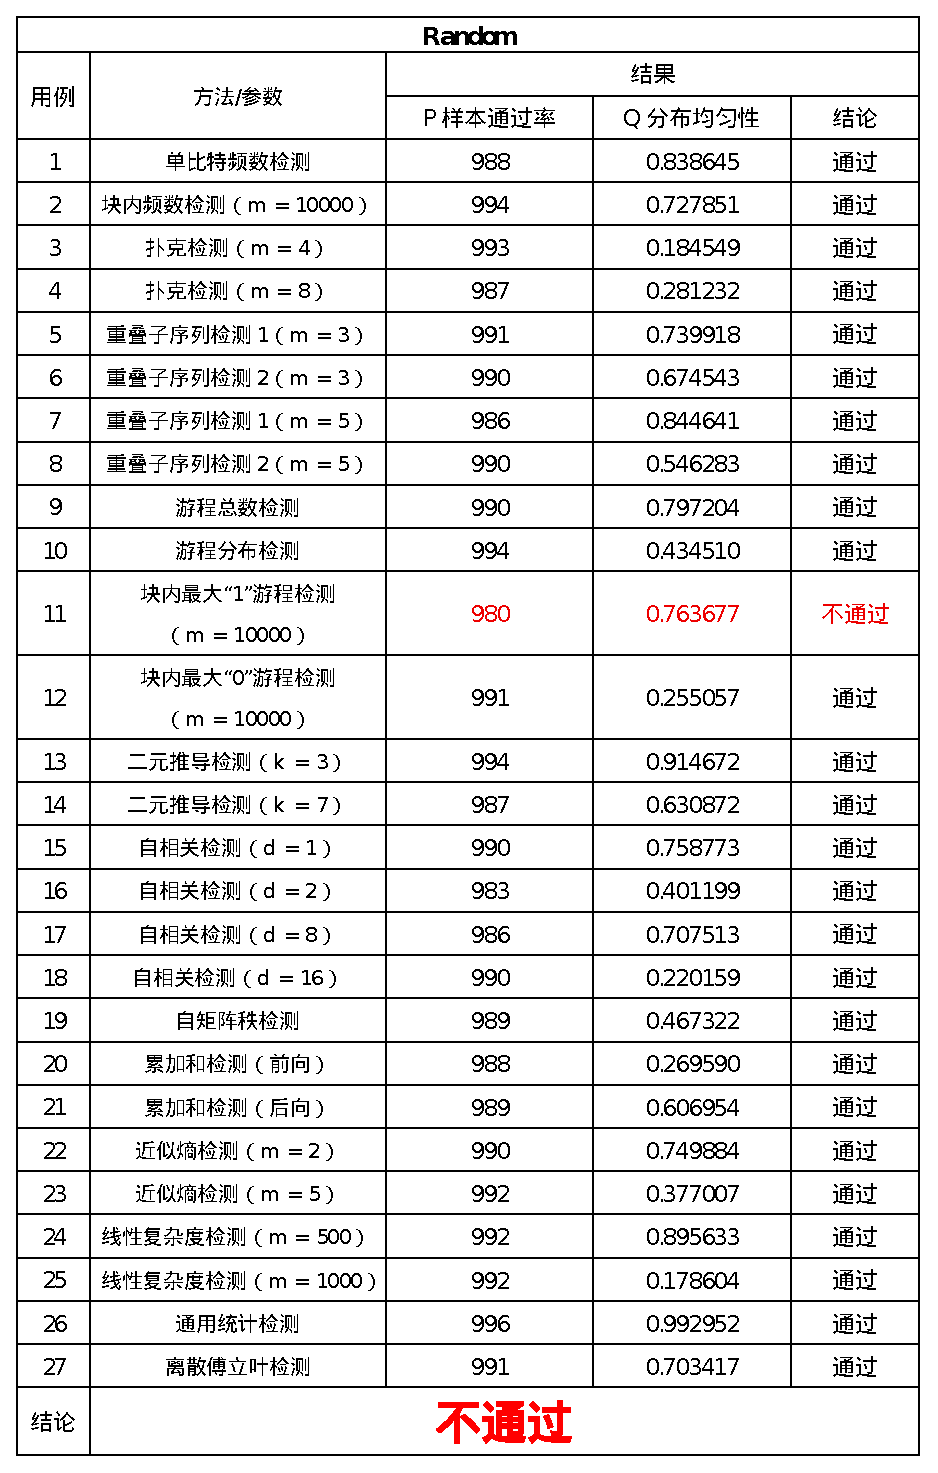
\includegraphics[width=\linewidth]{Random}
            \caption{Random 的运行结果}
            \label{fig:img4}
        \end{minipage}\hfill
        \begin{minipage}{0.42\textwidth}
            \centering
            \includegraphics[width=\linewidth]{RdRand}
            \caption{RdRand 的运行结果}
            \label{fig:img5}
        \end{minipage}\hfill
        \begin{minipage}{0.42\textwidth}
            \centering
            \includegraphics[width=\linewidth]{Random_k}
            \caption{Random 的斜率}
            \label{fig:img6}
        \end{minipage}\hfill
        \begin{minipage}{0.42\textwidth}
            \centering
            \includegraphics[width=\linewidth]{RdRand_k}
            \caption{RdRand 的斜率}
            \label{fig:img7}
        \end{minipage}
    \end{figure}

    \newpage
    由图可见,实验的结果符合理论推导,即在 Monte Calo 积分中,收敛的阶数为 \(O (N^{-1 / 2})\)。

    \section{结论}
    本文通过理论和代码的方式,验证了在 Monte Calo 积分中,收敛的阶数为 \(O (N^{-1 / 2})\),此结论亦可推广到任何 Monte Calo 方法中。不过本文并没有考虑到使用特殊的序列(即准随机),例如 Halton 序列、Sobol 序列和 Niederreiter 序列,这些序列由于其的固定顺序,导致了其并非独立多次的 Bernoulli 试验,无法使用以上理论公式。其在收敛的速度上会更快,斜率的绝对值会更大一些,针对该角度,有待后人更深入的研究。


\end{document}% 结束文档编辑,后面写啥都编译不出来
